\section{Curve Sketching}\label{sec:sketch}

We have been learning how we can understand the behavior of a function based on its first and second derivatives. While we have been treating the properties of a function separately (increasing and decreasing, concave up and concave down, etc.), we combine them here to produce an accurate graph of the function without plotting lots of extraneous points.

Why bother? Graphing utilities are very accessible, whether on a computer, a hand-held calculator, or a smartphone. These resources are usually very fast and accurate. We will see that our method is not particularly fast --- it will require time (but it is not \textit{hard}). So again: why bother?

\mtable{Demonstrating the 4 ways that concavity interacts with increasing/decreasing, along with the relationships with the first and second derivatives.}{fig:concavity3}{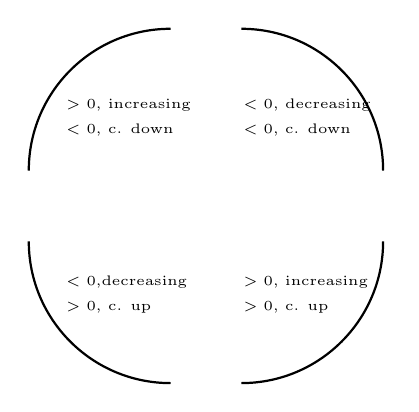
\begin{tikzpicture}[scale=.9]
\draw [thick] (-2.5,.5) arc (180:90:2);
\draw [thick] (2.5,.5) arc (0:90:2);
\draw [thick] (-2.5,-.5) arc (180:270:2);
\draw [thick] (2.5,-.5) arc (0:-90:2);
\draw(-1,1.25)node[]{\tiny\parbox{50pt}{$\fp>0$, increasing\\[3pt]$\fpp<0$, c. down}};
\draw(1.5,1.25)node[]{\tiny\parbox{50pt}{$\fp<0$, decreasing\\[3pt]$\fpp<0$, c. down}};
\draw(-1,-1.25)node[]{\tiny\parbox{50pt}{$\fp<0$,decreasing\\[3pt]$\fpp>0$, c. up}};
\draw(1.5,-1.25)node[]{\tiny\parbox{50pt}{$\fp>0$, increasing\\[3pt]$\fpp>0$, c. up}};
\end{tikzpicture}}

We are attempting to understand the behavior of a function $f$ based on the information given by its derivatives. While all of a function's derivatives relay information about it, it turns out that ``most'' of the behavior we care about is explained by \fp\ and \fpp. Understanding the interactions between the graph of $f$ and \fp\ and \fpp\ is important and is illustrated in \autoref{fig:concavity3}. To gain this understanding, one might argue that all that is needed is to look at lots of graphs. This is true to a point, but is somewhat similar to stating that one understands how an engine works after looking only at pictures. It is true that the basic ideas will be conveyed, but ``hands-on'' access increases understanding.

The following Key Idea summarizes what we have learned so far that is applicable to sketching graphs of functions and gives a framework for putting that information together. It is followed by several examples.

\ifthenelse{\boolean{latexml}}{%
% the key idea is long enough that it needs to be broken over two pages
% but not in html, where that doesn't matter
\keyidea{idea:sketch}{Curve Sketching}
{To produce an accurate sketch a given function $f$, consider the following steps.\index{curve sketching}
\begin{enumerate}
	\item	Find the domain of $f$. Generally, we assume that the domain is the entire real line then find restrictions, such as where a denominator is 0 or where negatives appear under the radical.
	\item	Find the location of any vertical asymptotes of $f$ (usually done in conjunction with the previous step).
	\item	Find the $x$ and $y$-intercepts of $f$, and any symmetry.
	\item	Consider the limits $\ds\lim_{x\to-\infty}f(x)$ and $\ds\lim_{x\to\infty}f(x)$ to determine the end behavior of the function.
	\item	Find the critical points of $f$.
	\item	Find the possible points of inflection of $f$.
	\item	Create a number line that includes all critical points, possible points of inflection, and locations of vertical asymptotes. For each interval created, determine whether $f$ is increasing or decreasing, concave up or down.
	\item	Evaluate $f$ at each critical point and possible point of inflection. Plot these points on a set of axes. Connect these points with curves exhibiting the proper concavity. Sketch asymptotes and $x$ and $y$-intercepts where applicable.
\end{enumerate}}%
}{%
\keyidea{idea:sketch}{Curve Sketching}
{To produce an accurate sketch a given function $f$, consider the following steps.\index{curve sketching}
\begin{enumerate}[series=curvesketching]
	\item	Find the domain of $f$. Generally, we assume that the domain is the entire real line then find restrictions, such as where a denominator is 0 or where negatives appear under the radical.
	\item	Find the location of any vertical asymptotes of $f$ (usually done in conjunction with the previous step).
	\item	Find the $x$ and $y$-intercepts of $f$, and any symmetry.
\end{enumerate}
\textit{\small(continued)}
}

\addtocounter{keyideaEnv}{-1}
%\renewcommand{\thmcontinues}[1]{Curve Sketching --- Continued}
%\keyidea[,continues=idea:sketch]{idea:sketchb}{Curve Sketching --- Continued}
\keyidea{idea:sketchb}{Curve Sketching --- Continued}
{~\\[-2\baselineskip]
\hspace{0pt}\begin{enumerate}[resume=curvesketching] % just resume doesn't cut it
	\item	Consider the limits $\ds\lim_{x\to-\infty}f(x)$ and $\ds\lim_{x\to\infty}f(x)$ to determine the end behavior of the function.
	\item	Find the critical points of $f$.
	\item	Find the possible points of inflection of $f$.
	\item	Create a number line that includes all critical points, possible points of inflection, and locations of vertical asymptotes. For each interval created, determine whether $f$ is increasing or decreasing, concave up or down.
	\item	Evaluate $f$ at each critical point and possible point of inflection. Plot these points on a set of axes. Connect these points with curves exhibiting the proper concavity. Sketch asymptotes and $x$ and $y$-intercepts where applicable.
\end{enumerate}}%
}

\youtubeVideo{DMYUsv8ZaoY}{Summary of Curve Sketching --- Example 2, Part 1 of 4}

\example{ex_sketch1}{Curve sketching}{Use \autoref{idea:sketch} to sketch $f(x) = 3x^3-10x^2+4x+10$.}
{We follow the steps outlined in the Key Idea.
\begin{enumerate}
	\item	The domain of $f$ is the entire real line; there are no values $x$ for which $f(x)$ is not defined.
	\item	There are no vertical asymptotes.
	\item	We see that $f(0)=10$, and $f$ does not appear to factor easily (so we skip finding the roots).  It has no symmetry.
	\item	We determine the end behavior using limits as $x$ approaches $\pm$infinity.			\[\lim_{x\to-\infty}f(x)=-\infty\qquad\lim_{x\to\infty}f(x)=\infty.\]
		We do not have any horizontal asymptotes.
	\item	Find the critical points of $f$. We compute $\fp(x) = 9x^2-20x+4=(9x-2)(x-2)$, so that $x=\frac29,2$.
	\item	Find the possible points of inflection of $f$. We see $\fpp(x) = 18x-20$, so that
	\[\fpp(x) = 0 \Rightarrow x= 10/9 \approx 1.111.\]
	\item	We place the values $x=\frac29,\frac{10}9,2$ on a number line. We mark each subinterval as increasing or decreasing, concave up or down, using the techniques used in Sections \ref{sec:incr_decr} and \ref{sec:concavity}.

\mtable{Sketching $f$ in \autoref{ex_sketch1}.}{fig:sketch1}{%
\begin{tikzpicture}
\begin{axis}[width=1.16\marginparwidth,tick label style={font=\scriptsize},minor x tick num=1,axis y line=middle,axis x line=middle,ymin=-.5,ymax=10.9,xmin=-1.2,xmax=3.2,name=myplot]
\addplot [draw={\colorone},thick,smooth] coordinates {(-.75,.109)(.222,10.428)(1.111,6.214)(2,2)(2.8,8.656)};
\filldraw [draw={\colorone},fill={\colorone}] (axis cs:0.222,10.428) circle (1pt);
\filldraw [draw={\colorone},fill={\colorone}] (axis cs:1.111,6.214) circle (1pt);
\filldraw [draw={\colorone},fill={\colorone}] (axis cs:2,2) circle (1pt);
\end{axis}
\node [right] at (myplot.right of origin) {\scriptsize $x$};
\node [above] at (myplot.above origin) {\scriptsize $y$};
\end{tikzpicture}\\
(a)\\
\begin{tikzpicture}
\begin{axis}[width=1.16\marginparwidth,tick label style={font=\scriptsize},minor x tick num=1,axis y line=middle,axis x line=middle,ymin=-.5,ymax=10.9,xmin=-1.2,xmax=3.2,name=myplot]
\addplot [draw={\colorone},smooth,thick,domain=-.75:2.8] {3*x^3-10*x^2+4*x+10};
\filldraw [draw={\colorone},fill={\colorone}] (axis cs:0.222,10.428) circle (1pt);
\filldraw [draw={\colorone},fill={\colorone}] (axis cs:1.111,6.214) circle (1pt);
\filldraw [draw={\colorone},fill={\colorone}] (axis cs:2,2) circle (1pt);
\end{axis}
\node [right] at (myplot.right of origin) {\scriptsize $x$};
\node [above] at (myplot.above origin) {\scriptsize $y$};
\end{tikzpicture}\\ (b)}

\begin{center}
\includecodegraphics{figures/matrices/sketch1}
\end{center}

	\item	We plot the appropriate points on axes as shown in \autoref{fig:sketch1}(a) and connect the points with the proper concavity. Our curve crosses the $y$ axis at $y=10$ and crosses the $x$ axis near $x=-0.75$. In \autoref{fig:sketch1}(b) we show a graph of $f$ drawn with a computer program, verifying the accuracy of our sketch.\eoehere
\end{enumerate}}

\example{ex_sketch2}{Curve sketching}{Sketch $\ds f(x) = \frac{x^2-x-2}{x^2-x-6}$.}
{We again follow the steps outlined in \autoref{idea:sketch}.

\begin{enumerate}
	\item	In determining the domain, we assume it is all real numbers and look for restrictions. We find that at $x=-2$ and $x=3$, $f(x)$ is not defined. So the domain of $f$ is $D = \{\text{real numbers } x\ \vert \ x\neq -2,3\}$.
		
	\item	The vertical asymptotes of $f$ are at $x=-2$ and $x=3$, the places where $f$ is undefined.  We see that $\ds\lim_{x\to-2^-}f(x)=\infty$, $\ds\lim_{x\to-2^+}f(x)=-\infty$, $\ds\lim_{x\to3^-}f(x)=-\infty$, and $\ds\lim_{x\to3^+}f(x)=\infty$.
		
	\item	We see that $f(0)=\frac13$ and that $f(x)=0$ when $0=x^2-x-2=(x-2)(x+1)$ so that $x=-1,2$.  There is no symmetry.

	\item	There is a horizontal asymptote of $y=1$, as $\ds \lim_{x\to -\infty}f(x) = 1$ and $\ds\lim_{x\to\infty}f(x) =1$.
		
	\item	To find the critical points of $f$, we first find $\fp(x)$. Using the Quotient Rule, we find
	\[\fp(x) = \frac{-8x+4}{(x^2+x-6)^2} = \frac{-8x+4}{(x-3)^2(x+2)^2}.\]
		
	$\fp(x) = 0$ when $x = 1/2$, and $\fp$ is undefined when $x=-2,3$. Since \fp\ is undefined only when $f$ is, these are not critical points. The only critical point is $x=1/2$.
		
	\item	To find the possible points of inflection, we find $\fpp(x)$, again employing the Quotient Rule:
	\[\fpp(x) = \frac{24x^2-24x+56}{(x-3)^3(x+2)^3}.\]
		
	We find that $\fpp(x)$ is never 0 (setting the numerator equal to 0 and solving for $x$, we find the only roots to this quadratic are imaginary) and \fpp\ is undefined when $x=-2,3$. Thus concavity will possibly only change at $x=-2$ and $x=3$ (although these are not inflection points, since $f$ is not defined there).
		
\mtable[-2in]{Sketching $f$ in \autoref{ex_sketch2}.}{fig:sketch2}{%
\begin{tikzpicture}
\begin{axis}[width=1.16\marginparwidth,tick label style={font=\scriptsize},
minor x tick num=1,minor y tick num = 4, axis y line=middle,axis x line=middle,
ymin=-5.5,ymax=5.5,xmin=-5.2,xmax=5.2,name=myplot]
\draw [draw={\colorone},thick] (axis cs:-5,1.2) parabola (axis cs:-2,10);
\draw [draw={\colorone},thick] (axis cs:3,9) parabola [bend at end] (axis cs:5,1.2);
\draw [draw={\colorone},thick,smooth] (axis cs:-1.8,-5) .. controls (axis cs:-1.7,-.5) .. (axis cs:-1,0) .. controls (axis cs:0,.36) .. (axis cs:.5,.36) .. controls (axis cs: 1,.36) .. (axis cs: 2,0) .. controls (axis cs:2.7,-.5) .. (axis cs:2.8,-5);
\addplot [thin,dashed] coordinates {(-2,5.5) (-2,-5.5)};
\addplot [thin,dashed] coordinates {(3,5.5) (3,-5.5)};
\addplot [thin,dashed] coordinates {(-5.5,1) (5.5,1)};
\filldraw [draw={\colorone}] (axis cs:0.5,.36) circle (1pt);
\end{axis}
\node [right] at (myplot.right of origin) {\scriptsize $x$};
\node [above] at (myplot.above origin) {\scriptsize $y$};
\end{tikzpicture}
\\[10pt](a)\\[10pt]
\begin{tikzpicture}
\begin{axis}[width=1.16\marginparwidth,tick label style={font=\scriptsize},
minor x tick num=1,minor y tick num = 4, axis y line=middle,axis x line=middle,
ymin=-5.5,ymax=5.5,xmin=-5.2,xmax=5.2,name=myplot]
\addplot [thick,draw={\colorone},smooth,domain=-5:-2.1] {((x-2)*(x+1))/((x-3)*(x+2))};
\addplot [thick,draw={\colorone},smooth,domain=-1.9:2.9] {((x-2)*(x+1))/((x-3)*(x+2))};
\addplot [thick,draw={\colorone},smooth,domain=3.1:5] {((x-2)*(x+1))/((x-3)*(x+2))};
\addplot [thin,dashed] coordinates {(-2,5.5) (-2,-5.5)};
\addplot [thin,dashed] coordinates {(3,5.5) (3,-5.5)};
\addplot [thin,dashed] coordinates {(-5.5,1) (5.5,1)};
\filldraw [draw={\colorone}] (axis cs:0.5,.36) circle (1pt);
\end{axis}
\node [right] at (myplot.right of origin) {\scriptsize $x$};
\node [above] at (myplot.above origin) {\scriptsize $y$};
\end{tikzpicture}
\\[10pt](b)}

	\item	We place the values $x=1/2$, $x=-2$ and $x=3$ on a number line. We mark in each interval whether $f$ is increasing or decreasing, concave up or down. We see that $f$ has a relative maximum at $x=1/2$; concavity changes only at the vertical asymptotes.

\begin{center}
\includecodegraphics{figures/matrices/sketch2}
\end{center}
		
	\item	In \autoref{fig:sketch2}(a), we plot the points from the number line on a set of axes and connect the points with the appropriate concavity. We also show $f$ crossing the $x$ axis at $x=-1$ and $x=2$. \autoref{fig:sketch2}(b) shows a computer generated graph of $f$, which verifies the accuracy of our sketch.\eoehere
\end{enumerate}}

\example{ex_sketch3}{Curve sketching}{Sketch $\ds f(x) = \frac{5(x-2)(x+1)}{x^2+2x+4}.$}
{We again follow \autoref{idea:sketch}.
	\begin{enumerate}
	\item	We assume that the domain of $f$ is all real numbers and consider restrictions. The only restrictions come when the denominator is 0, but this never occurs. Therefore the domain of $f$ is all real numbers, $\mathbb{R}$.
	\item	There are no vertical asymptotes.
	\item	We see that $f(0)=-\dfrac52$ and that $f(x)=0$ when $x=-1,2$.
	\item	We have a horizontal asymptote of $y=5$, as
	\[\lim_{x\to\pm\infty}f(x)=\lim_{x\to\pm\infty}\frac{5(1-\frac2x)(1+\frac1x)}{1+\frac2x+\frac4{x^2}}=5.\]
	\item	We find the critical points of $f$ by setting $\fp(x)=0$ and solving for $x$. We find 
	\[
	\fp(x) = \frac{15x(x+4)}{(x^2+2x+4)^2}
	\quad \Rightarrow \quad
	\fp(x) = 0 \text{ when } \ x=-4,0.
	\]
	\item	We find the possible points of inflection by solving $\fpp(x) = 0$ for $x$. We find
	\[\fpp(x) = -\frac{30x^3+180x^2-240}{(x^2+2x+4)^3}.\]
	The cubic in the numerator does not factor very ``nicely.'' We instead approximate the roots at $x= -5.759$, $x=-1.305$ and $x=1.064$.
			
	\item	We place the critical points and possible inflection points on a number line and mark each interval as increasing/decreasing, concave up/down appropriately.

\begin{center}
\includecodegraphics{figures/matrices/sketch3}
\end{center}	
	
\mtable{Sketching $f$ in \autoref{ex_sketch3}.}{fig:sketch3}{%
\begin{tikzpicture}
\begin{axis}[width=1.16\marginparwidth,tick label style={font=\scriptsize},
minor x tick num=1, axis y line=middle,axis x line=middle,
ymin=-3.1,ymax=8.1,xmin=-7.5,xmax=6.5,name=myplot]
\addplot [thin,dashed] coordinates {(-7.5,5) (6.5,5)};
\draw [draw={\colorone},thick]  (axis cs:-7,6.1)parabola (axis cs:-5.75,7.2);
\draw [draw={\colorone},thick]  (axis cs:-5.75,7.2)parabola[bend at end](axis cs:-4.,7.5);
\draw [draw={\colorone},thick]  (axis cs:-4., 7.5) parabola (axis cs:-1.31, 1.63);
\draw [draw={\colorone},thick]  (axis cs:-1.31, 1.63) -- (axis cs:-1,0);
\draw [draw={\colorone},thick]  (axis cs:-1,0) parabola [bend at end] (axis cs:0., -2.5);
\draw [draw={\colorone},thick]  (axis cs:0.,-2.5) parabola (axis cs:1.064, -1.33);
\addplot [draw={\colorone},thick,smooth] coordinates {(1.064, -1.33049) (1.264, -1.02533) (1.464, -0.727958) (1.664,-0.443257) (1.864, -0.173847) (2,0)};
\draw [draw={\colorone},thick]  (axis cs:2,0) parabola [bend at end] (axis cs:6,4.5);
\filldraw [draw={\colorone}] (axis cs:-5.75,7.2) circle (1pt);
\filldraw [draw={\colorone}] (axis cs:-4., 7.5) circle (1pt);
\filldraw [draw={\colorone}] (axis cs:-1.31, 1.63) circle (1pt);
\filldraw [draw={\colorone}] (axis cs:-1,0) circle (1pt);
\filldraw [draw={\colorone}] (axis cs:0., -2.5) circle (1pt);
\filldraw [draw={\colorone}] (axis cs:1.064, -1.33) circle (1pt);
\filldraw [draw={\colorone}] (axis cs:2,0) circle (1pt);\end{axis}
\node [right] at (myplot.right of origin) {\scriptsize $x$};
\node [above] at (myplot.above origin) {\scriptsize $y$};
\end{tikzpicture}
\\[10pt](a)\\[10pt]
\begin{tikzpicture}
\begin{axis}[width=1.16\marginparwidth,tick label style={font=\scriptsize},
minor x tick num=1, axis y line=middle,axis x line=middle,
ymin=-3.1,ymax=8.1,xmin=-7.5,xmax=6.5,name=myplot]
\addplot [thin,dashed] coordinates {(-7.5,5) (6.5,5)};
\addplot [thick,draw={\colorone},smooth,domain=-7.5:6.5] {(5*(x-2)*(x+1))/(x^2+2*x+4)};
\filldraw [draw={\colorone}] (axis cs:-5.75,7.2) circle (1pt);
\filldraw [draw={\colorone}] (axis cs:-4., 7.5) circle (1pt);
\filldraw [draw={\colorone}] (axis cs:-1.31, 1.63) circle (1pt);
\filldraw [draw={\colorone}] (axis cs:-1,0) circle (1pt);
\filldraw [draw={\colorone}] (axis cs:0., -2.5) circle (1pt);
\filldraw [draw={\colorone}] (axis cs:1.064, -1.33) circle (1pt);
\filldraw [draw={\colorone}] (axis cs:2,0) circle (1pt);
\end{axis}
\node [right] at (myplot.right of origin) {\scriptsize $x$};
\node [above] at (myplot.above origin) {\scriptsize $y$};
\end{tikzpicture}
\\[10pt](b)}

	\item	In \autoref{fig:sketch3}(a) we plot the significant points from the number line as well as the two roots of $f$, $x=-1$ and $x=2$, and connect the points with the appropriate concavity. \autoref{fig:sketch3}(b) shows a computer generated graph of $f$, affirming our results (but the top left was slightly off).\eoehere
\end{enumerate}}

In each of our examples, we found a few, significant points on the graph of $f$ that corresponded to changes in increasing/decreasing or concavity. We connected these points with curves, and finished by showing a very accurate, computer generated graph. 

Why are computer graphics so good? It is not because computers are ``smart\-er'' than we are. Rather, it is largely because computers are much faster at computing than we are. In general, computers graph functions much like most students do when first learning to draw graphs: they plot equally spaced points, then connect the dots using lines. By using lots of points, the connecting lines are short and the graph looks smooth. 

This does a fine job of graphing in most cases (in fact, this is the method used for many graphs in this text). However, in regions where the graph is very ``curvy,'' this can generate noticeable sharp edges on the graph unless a large number of points are used. High quality computer algebra systems, such as \textit{Mathematica}, use special algorithms to plot lots of points only where the graph is ``curvy.''

In \autoref{fig:mathematica_sinx}, a graph of $y=\sin x$ is given, generated by \textit{Mathematica}. The small points represent each of the places \textit{Mathematica} sampled the function. Notice how at the ``bends'' of $\sin x$, lots of points are used; where $\sin x$ is relatively straight, fewer points are used. (Many points are also used at the endpoints to ensure the ``end behavior'' is accurate.) 

\begin{figure}[!ht]
\centering
\includegraphics{figures/raw/figmathematica_sinx}
\caption{A graph of $y=\sin x$ generated by \textit{Mathematica}.}
\label{fig:mathematica_sinx}
\end{figure}

How does \textit{Mathematica} know where the graph is ``curvy''? Calculus. When we study \textit{curvature} in a later chapter, we will see how the first and second derivatives of a function work together to provide a measurement of ``curviness.'' \textit{Mathematica} employs algorithms to determine regions of ``high curvature'' and plots extra points there.

Again, the goal of this section is not ``How to graph a function when there is no computer to help.'' Rather, the goal is ``Understand that the shape of the graph of a function is largely determined by understanding the behavior of the function at a few key places.'' In \autoref{ex_sketch3}, we were able to accurately sketch a complicated graph using only 5 points and knowledge of asymptotes!

There are many applications of our understanding of derivatives beyond curve sketching. The next chapter explores some of these applications, demonstrating just a few kinds of problems that can be solved with a basic knowledge of differentiation. 

\printexercises{exercises/03_05_exercises}

% todo write more problems
